%%%%%%%%%%%%%%%%%%%%%%%%%%%%%%%%%%%%%%%%%%%%%%%%%%%%%%%%%%%%%%%%%%
%%%%%%%% ICML 2014 EXAMPLE LATEX SUBMISSION FILE %%%%%%%%%%%%%%%%%
%%%%%%%%%%%%%%%%%%%%%%%%%%%%%%%%%%%%%%%%%%%%%%%%%%%%%%%%%%%%%%%%%%

% Use the following line _only_ if you're still using LaTeX 2.09.
%\documentstyle[icml2014,epsf,natbib]{article}
% If you rely on Latex2e packages, like most moden people use this:
\documentclass{article}

% use Times
\usepackage{times}
% For figures
\usepackage{graphicx} % more modern
%\usepackage{epsfig} % less modern
%\usepackage{subfigure}

% For citations
\usepackage{natbib}

% For algorithms
\usepackage{algorithm}
\usepackage{algorithmic}

% As of 2011, we use the hyperref package to produce hyperlinks in the
% resulting PDF.  If this breaks your system, please commend out the
% following usepackage line and replace \usepackage{icml2014} with
%\usepackage[nohyperref]{icml2014} above.
\usepackage{hyperref}

% Packages hyperref and algorithmic misbehave sometimes.  We can fix
% this with the following command.
\newcommand{\theHalgorithm}{\arabic{algorithm}}

% Employ the following version of the ``usepackage'' statement for
% submitting the draft version of the paper for review.  This will set
% the note in the first column to ``Under review.  Do not distribute.''
\usepackage[accepted]{icml2014} 


% The \icmltitle you define below is probably too long as a header.
% Therefore, a short form for the running title is supplied here:
\icmltitlerunning{Objects Recognization Based on SOG with SVM}

\begin{document} 

\twocolumn[
\icmltitle{Objects Recognization Based on SOG with SVM\\Final Report for CIS 519}

% It is OKAY to include author information, even for blind
% submissions: the style file will automatically remove it for you
% unless you've provided the [accepted] option to the icml2014
% package.
\icmlauthor{Shangyi Cheng}{shangyi@seas.upenn.edu}
\icmlauthor{Yao Chu}{chuyao@seas.upenn.edu}
\icmlauthor{Chenyang Zhao}{chzhao@seas.upenn.edu}

% You may provide any keywords that you 
% find helpful for describing your paper; these are used to populate 
% the "keywords" metadata in the PDF but will not be shown in the document
\icmlkeywords{machine learning, circle detection, feature extraction, objects recognization, neural network}

\vskip 0.3in
]

\begin{abstract} 
We studied the question of object recognization using histograms of oriented gradients (HOG) and support vector machine (SVM) with Gaussian Kernel on ball detection as a test case. After reviewing several existing methods for feature extraction, our project verified that HOG performs well in ball recognization. The whole process is shown in this report, from choosing regions of interest manually, extracting features from these regions using HOG, using principal component analysis (PCA) to reduce dimension of the  dataset and then applying SVM with Gaussian kernel to classify.   
\end{abstract}


\section{Introduction}
The topic for this project is to detect the object of our interest on the given images and predict which class it belongs to. The dataset we use is from Caltech 256(Griffin, G. Holub, AD. Perona, P.), which contain images of four kinds of balls, including 98 images of golf in the folder ``088.golf-ball'', 174 images of soccer ball in ``193.soccer-ball'', 104 images of bowling-ball in ``017.bowling-ball'' and 98 images of tennis ball in ``216.tennis-ball''. As shown in Figure \cite{ROIResult}, among images of the same kind (take soccer-ball as example), some of the images have a whole contour of soccer in the center and fill the image, while in other images(such as a photo of a soccer game), the soccer may cover a small portion in the corner, or only part of a soccer or a group of soccers appear on the image. We decide to use the image with a single target occupying most of the image as the training set. So the first thing we need to do before training is to create such standard images for training from the raw dataset. And our final goal is, given a new image,  the model can detect whether this image contains any ball of our interest or just unrelated to balls and in the first condition, the model can give the label for the class the detected object belongs to.

\section{Model Details} 

\subsection{Overview of the Method}
Inspired by the paper \cite{dalal2005histograms} presented by Navneet Dalal and Bill Triggs, we tried the method described in this paper. The summary figure for our approch is shown in Figure .\\
An overview of the whole process is shown in Figure \cite{overview}.\\
For the training process, we first preprocess the images by selecting the region containing the ball manually, resize and restore such images as the dataset for feature extraaction. Then, HOG is applied on those processes images and get a vector of length $900$ as features for one instance. Thus, we build the training dataset, a .dat file. Then, SVM with Gaussian kernel is used to learn from the dataset. The metrics of accuracy, ROC and learning curve along with cross-validation are used to ensure that the model has learned to classify four kinds of balls with an acceptable accuracy without overfitting. The training is finished. \\
For the test part, given an brand-new image, no matter whether it contains any ball of our interest, what the portion of the ball covers the image and whether it appears in the center or in the corner, individually or in group, the model scan the image using mask with increasing size, doing the corresponding manipulation with the same parameters as those for training set, and then make prediction for each block. Among all predictions, the model will choose the ones with high confidence and decide whether they point to the same object. Finally, the target of our interest will be framed in a rectangle along with its label.

\begin{figure}[htp]
\centering
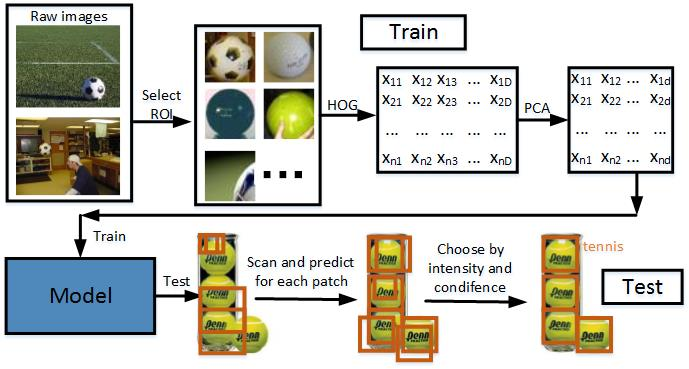
\includegraphics[width=0.5\textwidth]{overview.jpg}
\caption{An illustration of HOG with SVM process.}
\label{fig:overview}
\end{figure}

\subsection{Region of Interest (ROI) Selection}
Before we use HOG to extract features from labeled images, we need to select the ROI which contains an object we would like our model to recognize. We tried several ways to select such region.\\
At the beginning, we considered using corner detection directly on the original image to select ROI and at the same time extract features. However, as shown in Figure \cite{crd}, extracting corner features based on the Harris Corner Detection and Adaptive Non-maximal Suppression method \cite{brown2005multi} is not so helpful for following reasons: firstly, different pattern can be found in a single kind of balls so that geometric corner feature doesn't provide enough information for classification; secondly, the complicated background may generate large amount of features which are irrelevant to the ball.\\


\begin{figure}[htp]
\centering
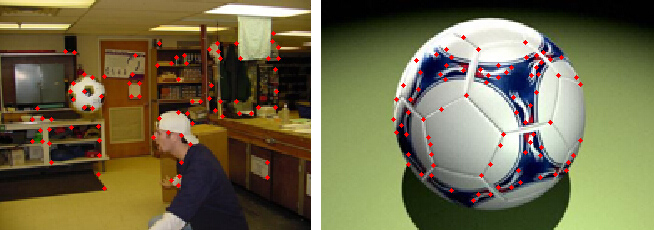
\includegraphics[width=0.4\textwidth]{CornerDetection.jpg}
\caption{Corner Detection Results}
\label{fig:crd}
\end{figure}

Then we tried several methods for circle detection including \cite{cirDetect1}, \cite{cirDetect2}, \cite{cirDetect3} to pick up the circular region and build the training set. One of the robustest approach is Circle Hough Transform (CHT), which takes the image $M$ and desired radius range $[r_{min},r_{max}]$ as inputs and return the positions of circle centers. As shown in Figure \cite{cird}, this method preforms good for the standard images with a single ball occupyting the whole image but has a poor performance when there are other ball-like distractions such as heads and the three holes on a bowling-ball, or only partial of the object, rather than a whole circle, appear on the image. It's also possible for CHT to return some position with high confidence for some circular patterns inside the ball. It's really hard to pick up the ROI just by the circular shape and without any referring to the patterns and features inside the region. \\

\begin{figure}[htp]
\centering
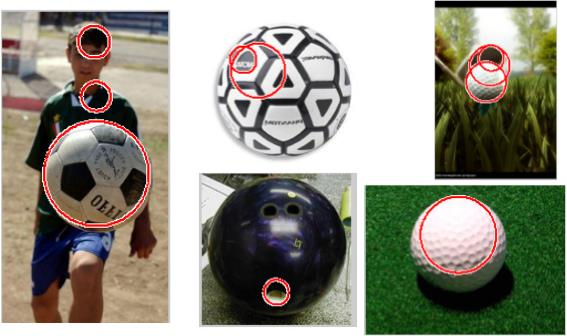
\includegraphics[width=0.4\textwidth]{circleDetection.jpg}
\caption{Unseccessful CHT Detection Results}
\label{fig:cird}
\end{figure}

Thus, we finally decided to select ROI for each image in dataset manually. To increase the number of instances in our training data, for each image, let the user chooses the ROI with a movable, resizable rectangle and position it interactively using the mouse. And then shift the area a little in one of the eight directions, thus a raw image will create at most nine images and at least one image for training. Finally, the picked area is resized to a $40 \times 40$ pixal square. Apart from the four kinds of balls, we also generate some squares with the label "Unknown" to represent the unrelated features to ball. The images in this class are mostly selected from the background, fragments of the ball and other unrelated area. Figure \cite{ROIResult} shows the processed images after manual selection and resize. First two rows are images for balls and the third row is for "Unknown".
\begin{figure}[htp]
\centering
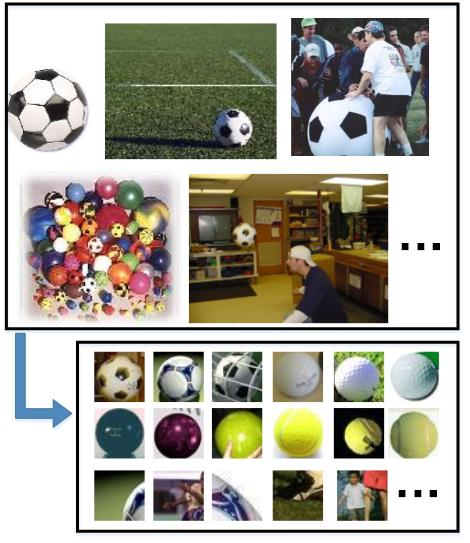
\includegraphics[width=0.4\textwidth]{ROISelection.jpg}
\caption{Resized Images Before \& After ROI Selection}
\label{fig:ROIResult}
\end{figure}

%%%%%%%%%%%%%%%%%%%%%%%%%%%%%%%%%%%%%%
\subsection{Histogram of Oriented Gradients Discriptors}
As described in ROI selection section, the patches cropped out manually were resized to 40x40 pixels. Each patch works as an dataset instance, however, there are two primary ways to extract features from these patches. First, each pixels value (grayscale, RGB or LAB color spaces) can be extracted directly as a feature. Second, apply HOG or SIFT to extract features. Considering the HOG/SIFT representation can capture edges and gradient structure which is characteristic of local shape as well as easily maintain the invariance to local geometric and photometric transformation, we finally chose second method. Also, HOG method can be implemented easily with fewer features compared to SIFT, so we chose to use HOG discriptors.\\  

Implementing HOG to extract features from patches followed procedure shown in figure \ref{fig:HOG}. For balls detection and classifier, following coefficient were chosen: All patches were converted into grayscale color space to normalize gamma and color; 1-D point derivative(centered [-1, 0, 1]) mask with no smoothing was applied to patches; 9 orientation bins evenly spaced over 0–
180 degrees (“unsigned” gradient) was chosen; Cell size 6x6 and block size 2x2 were choosen for R-HOG.  
\begin{figure}[htp]
\centering
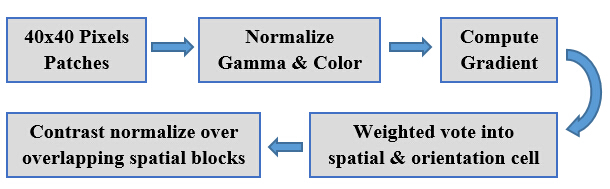
\includegraphics[width=0.4\textwidth]{HOG.jpg}
\caption{HOG Procedure}
\label{fig:HOG}
\end{figure}

HOG features is shown in figure \ref{fig:HOGtest}. After extract HOG features from a patch, reshape the feature matrix into a vector represent the patch. Eventually we generated a 3660x900 datasets with 3660 instances and 900 features. 

\begin{figure}[htp]
\centering
\includegraphics[width=0.4\textwidth]{HOGtest.jpg}
\caption{HOG Feature Extraction Result}
\label{fig:HOG}
\end{figure}

%%%%%%%%%%%%%%%%%%%%%%%%%%%%%%%%%%%%%%%
\subsection{PCA}
The number of features we get using HOG is $900$. Since the number of instances we use is about $4000$, which is not large enough for $900$ features and easy to result in overfit. On the other hand, to improve efficiency and decrease the time for training, it's necessary to reduce the dimension first. On the training dataset, we compute covariance matrix $\Sigma$ and mean (average over all rows of $X$). Next, we choose the $d$ most important PCA basis vectors as the new training dataset. Then $\Sigma$ and $X$ got previously on training dataset should be used on the test data.



%The algorithm is presented in Algorithm \ref{alg:Patch}.
%\begin{algorithm}[tb]
%   \caption{Select ROI Manually}
%   \label{alg:Patch}
%\begin{algorithmic}
%   \STATE {\bfseries Input:} image $I$
%   \STATE Initialize accumulator matrix $M = 0$.
%   \FOR{each edge point$(i,j)$ in image $I$}
%   \FOR{each point $(m,n)$ in image $I$}
%   \IF{$r_{min}^2<(m-i)^2+(n-j)^2<r_{max}^2$}
%   \STATE {$M(m,n) = M(m,n)+\phi_{m,n}$}
%   \ENDIF
%   \ENDFOR
%   \ENDFOR
%   \STATE {\bfseries Return:} positions of local maximum points in accumulator matrix $M$
%\end{algorithmic}
%\end{algorithm}\\

\subsection{Detect Balls from New Image}
Once classifier was trained, balls could be detected from the new input image based on the predict results. \\
In order to detect the balls, the algorithm should search every possible detect window in the image. So square detect window with changeable size move around in the image to extract test patches. Window size changes from minimum value (80 pixels or 10 percent of maximum side) to maximum value ( small one between image width and height). And overlapping ratio between two consecutive detect windows is 85 percent.  Every patch is resized to 40x40 pixels, extracted HOG features, and normalized in the same way with training data. Following this, apply classifier to predict labels for test instances. Based on the predict results, overlap test instances can be eliminated by adaptive non-maximum suppression. A neighbour positive detection threshold is set to improve the detection result. 
 


\section*{Acknowledgments} 
This project is supported by Uenn CIS 519. Thanks Eric Eaton and Xiaoxiang Hu for their instruction. Thanks MATLAB for providing so many useful toolboxes.

\bibliography{report-ChengChuZhao}
\bibliographystyle{icml2014}

\end{document} 


